\documentclass[11pt]{article}
\usepackage[utf8]{inputenc}
\usepackage[french]{babel}
\usepackage[margin=1in]{geometry}
\usepackage{amsfonts, amsmath, amssymb}
\usepackage[none]{hyphenat}
\usepackage{fancyhdr}
\usepackage{graphicx}
\usepackage{float}
\usepackage[nottoc, notlot, notlof]{tocbibind}
\usepackage{array,multirow,makecell}
\setcellgapes{1pt}
\makegapedcells
\usepackage[table]{xcolor}

\pagestyle{fancy}
\fancyhead{}
\fancyfoot{}
\fancyhead[L]{\slshape \MakeUppercase{Étude d’un MRUA}}
\fancyhead[R]{\slshape {Romain Blondel, Julien Bricka}}
\fancyfoot[C]{\thepage}
\renewcommand{\footrulewidth}{0pt}

\def \hfillx {\hspace*{ -\textwidth} \hfill}

\begin{document}

\begin{titlepage}
\begin{center}
\vspace{1cm}
\vfill
\line(1,0){400}\\
\huge{\textbf{Étude d’un mouvement rectiligne
uniformément accéléré}}\\
\line(1,0){400}\\
\vfill
\vfill
\begin{figure}[H]
  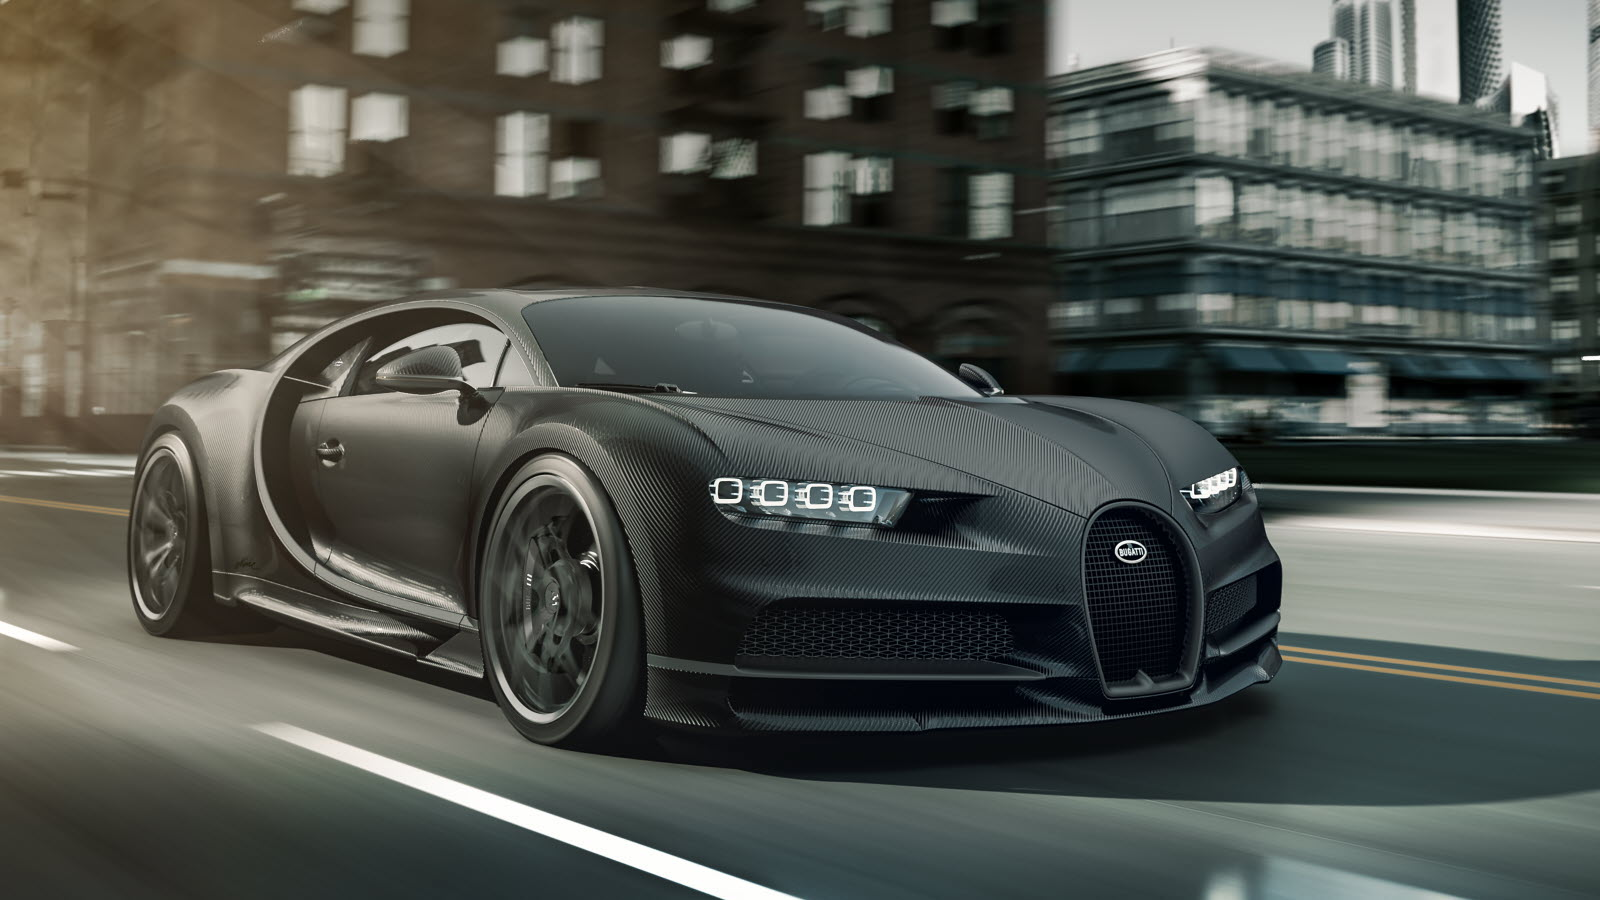
\includegraphics[scale=0.3]{la-voiture-noire-de-bugatti-modele-unique-photo-dr-1608828241.jpg}
\end{figure}
\vfill
Romain Blondel, Julien Bricka\\
1M8, Gymnase Auguste Piccard\\
\today
\end{center}
\end{titlepage}

\tableofcontents
\clearpage

\setcounter{page}{1}

\section{But}
Étudier un mouvement rectiligne uniformément accéléré (MRUA) sur une table inclinée.

\section{Introduction}
Les principaux outils théoriques que nous allons utiliser sont ceux concernant le MRUA. D’autres notions peuvent néanmoins être nécessaire tel que des règles simples de proportionnalité comme la règle de trois. Il faut malgré tout remarquer qu’une expérience, aussi précise soit-elle, ne reproduira pas les conditions exactes indispensables à la précision de la théorie. Cela reste la plus pratique pour étudier cette  expérience.
Donc, en quoi consiste le MRUA. Tout d’abord, les notions principales sont :
\begin{itemize}
    \item La distance $d$ en $[m]$ qui est une variation de positions $x_n$ tel que $d=x_b-x_a$ 
    \item Le temps $t$ en $[s]$
    \item La vitesse $v=\dfrac{d}{t}$ en $\left[\dfrac{m}{s} \right] $ 
    \item L’accélération $a=\dfrac{v}{t}$ en $\left[\dfrac{m}{s^2} \right] $ 
\end{itemize}
Il faut néanmoins garder à l’esprit que nous calculons une vitesse ou une accélération moyenne car par définition, la vitesse est la variation de distance ($\Delta x = x_2-x_1$) dans un intervalle de temps ($\Delta t = t_2-t_1$) et l’accélération, la variation de vitesse ($\Delta v = v_2-v_1$) dans le temps. Il est donc plus juste d’écrire :\\
 \begin{center}
 $v_m =\dfrac{\Delta x}{\Delta t} $ ainsi que $a_m =\dfrac{\Delta v}{\Delta t} $
 \end{center} 
D’où, pour avoir une $v$ ou a en un temps instantané, il faudrait avoir $ \Delta t$ le plus petit possible (ce qui est moins utile pour $a$ dans le MRUA car c’est une constante), soit :\\
\begin{center}
 $v(t)=\lim\limits_{\Delta t \to 0} \dfrac{\Delta x}{\Delta t} $ et $a =\lim\limits_{\Delta t \to 0} \dfrac{\Delta v}{\Delta t}$ \\
\textit{donc $v$ est la dérivée (ou la tangente) de $x$ en $t$ et $a$ la dérivée de $v$ en $t$}\\
 \end{center} 
De ces notions, on en tire l’équation horaire de la vitesse et de la distance ou de la position :
\begin{center}
$a=constante $\\
$v(t)= v_0+a \cdot t $\\
$x(t)-x_0=v_0 \cdot t + \dfrac{1}{2} \cdot a \cdot t^2 $ ou $x(t)=x_0+v_0 \cdot t + \dfrac{1}{2} \cdot a \cdot t^2 $
\end{center} 
qui forment les bases du MRUA.
\clearpage

\section{Démarche}
\subsection{Liste du matériel}
\subsubsection*{Pour l'expérience}
\begin{itemize}
    \item Palet avec ampoule dessus
    \item Deux ampoules séparées d’une distance fixe
    \item Table à coussin d’air avec élévations
    \item Filet et amortisseur autour de la table pour ne pas abîmer le palet
\end{itemize}

    
\subsubsection*{Pour la mesure}
\begin{itemize}
    \item Camera
    \item Disque monté sur un moteur rotatif avec deux ouvertures et une pastille réfléchissante
    \item Stroboscope
    \item Support pour la camera, perpendiculaire à la table
\end{itemize}
    
\subsection{Schéma du montage}
\begin{center}
\begin{figure}[H]
  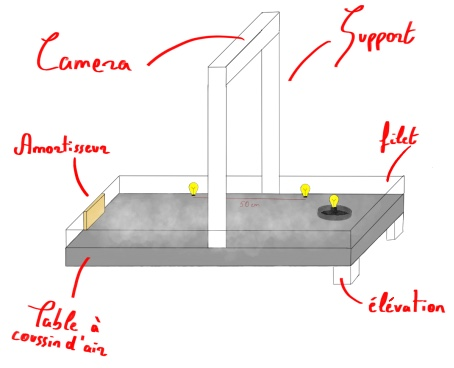
\includegraphics[scale=0.6]{side view2.jpg}
  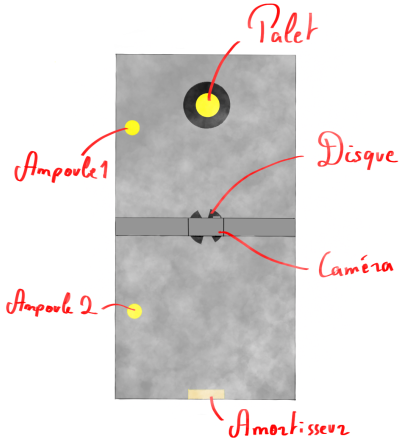
\includegraphics[scale=0.75]{front view.png}
  \begin{center}
    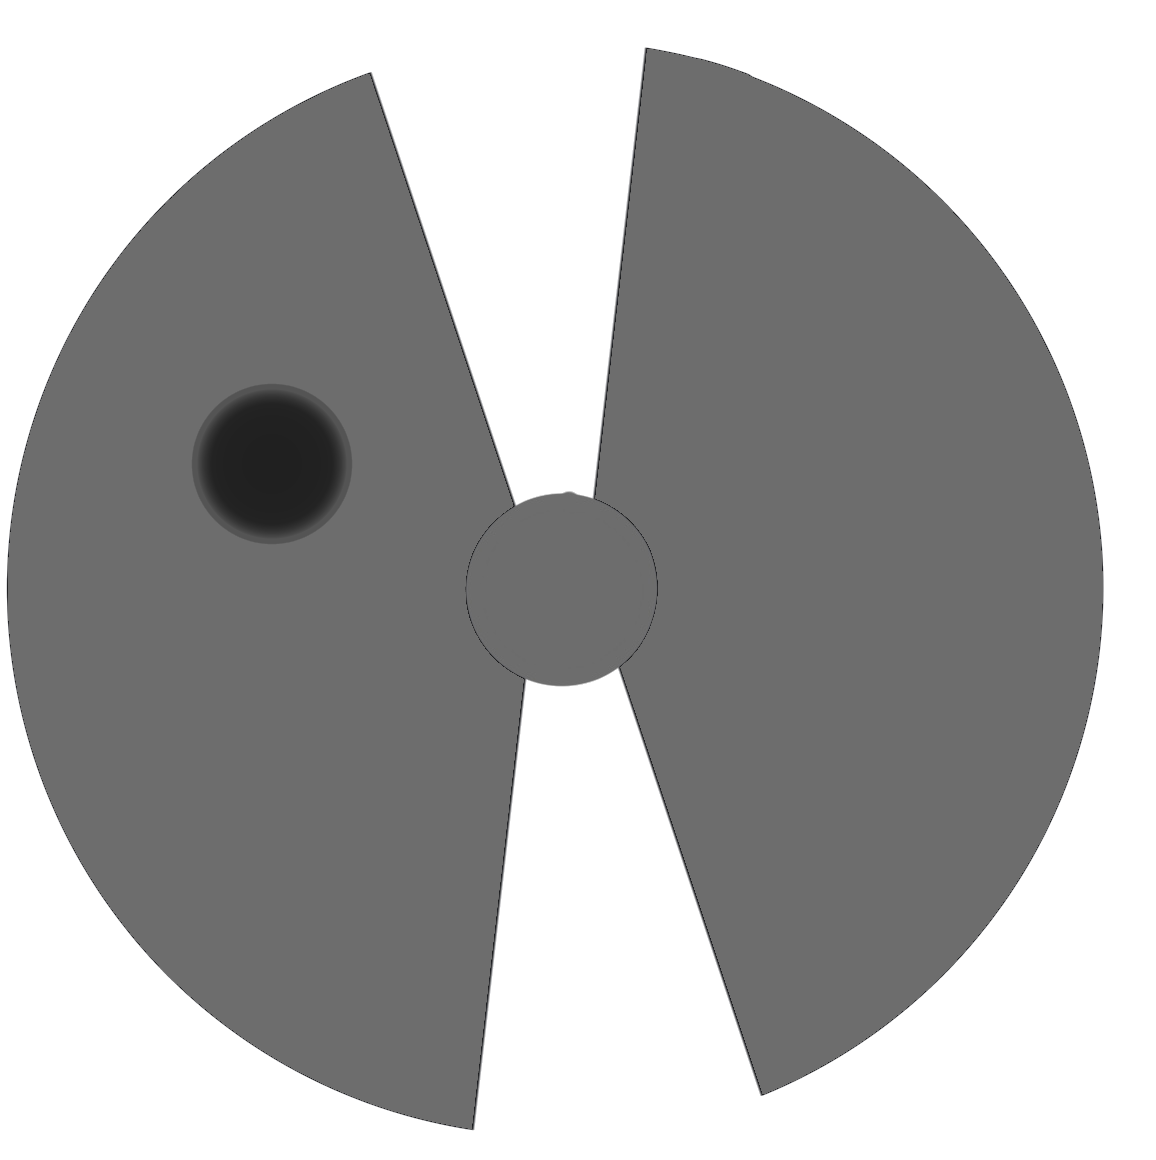
\includegraphics[scale=0.075]{circle.png} 
  \end{center}
  \caption{Vue de profil, du dessus et du disque avec la pastille réfléchissante (en noir)}	
\end{figure}
\end{center}
\clearpage

\subsection{Marche à suivre}
\begin{enumerate}
     \item Surélever avec les élévations un côté et enclencher la table à coussin d’air ainsi que les divers ampoules et paramétrer la camera afin d’avoir une pose longue (la pose doit durer tout le long de l’expérience).
     \item Mesurer la vitesse de rotation du disque. Pour ce faire, dans l’obscurité, ajuster la fréquence du stroboscope afin d’avoir l’illusion que la pastille réfléchissante soit statique. La moitié de cette fréquence correspond à l’intervalle de temps entre deux points.
     \item Commencer la photo de la camera en lâchant le palet en même temps.
     \item Traiter l’image obtenue afin d’inverser les couleurs et les accentuer.
     \item Relever les distance sur l’image depuis un point choisi arbitrairement.
\end{enumerate}
\begin{center}
\begin{figure}[H]
  \fbox{
  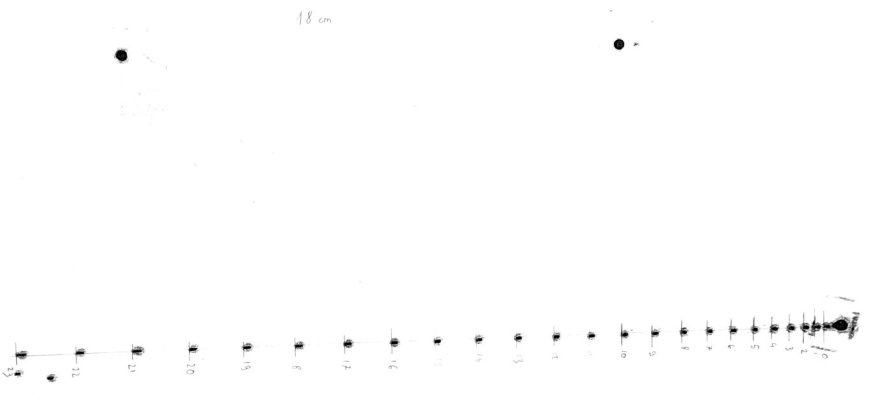
\includegraphics[scale=0.75]{Scan2.png}  }
  \caption{Scan de l'image ayant servi aux mesures}
\end{figure}
\end{center}
\textit{Note : dans les tableaux qui suivent, les distance sur l’image sont nommées $d$ et celles dans la réalité $x$, le temps $t$ et la vitesse moyenne au point $v_m$.}

    
\section{Résultats}
\subsection{Tableaux}
   \begin{table}[H]
        \begin{minipage}{0.5\textwidth}
            \centering
            \begin{center}
            \textbf{\caption{Distance des points sur \\l’image et dans la réalité}}
            \end{center}
			\begin{tabular}{ |>{\columncolor{lightgray}} l | l |>{\columncolor{lightgray}} l | l | }
				\hline
				\rowcolor{gray} point & $t [s]$ & $d [cm]$ & $x [m]$ \\ \hline \hline
				0 & 0.000 & 0.0 & 0.000 \\ \hline
				1 & 0.036 & 0.3 & 0.008 \\ \hline
				2 & 0.071 & 1.0 & 0.028 \\ \hline
				3 & 0.107 & 1.2 & 0.033 \\ \hline
				4 & 0.143 & 1.7 & 0.047 \\ \hline
				5 & 0.179 & 2.5 & 0.069 \\ \hline
				6 & 0.214 & 3.3 & 0.092 \\ \hline
				7 & 0.250 & 4.1 & 0.114 \\ \hline
				8 & 0.286 & 5.1 & 0.142 \\ \hline
				9 & 0.321 & 6.1 & 0.169 \\ \hline
				10 & 0.357 & 7.2 & 0.200 \\ \hline
				11 & 0.393 & 8.4 & 0.233 \\ \hline
				12 & 0.429 & 9.6 & 0.267 \\ \hline
				13 & 0.464 & 11.0 & 0.306 \\ \hline
				14 & 0.500 & 12.5 & 0.347 \\ \hline
				15 & 0.536 & 14.0 & 0.389 \\ \hline
				16 & 0.571 & 15.6 & 0.433 \\ \hline
				17 & 0.607 & 17.3 & 0.481 \\ \hline
				18 & 0.643 & 19.1 & 0.531 \\ \hline
				19 & 0.679 & 21.0 & 0.583 \\ \hline
				20 & 0.714 & 22.9 & 0.636 \\ \hline
				21 & 0.750 & 24.9 & 0.692 \\ \hline
				22 & 0.786 & 27.0 & 0.750 \\ \hline
				23 & 0.821 & 29.1 & 0.808 \\ \hline
			\end{tabular}       
        \end{minipage}
        \hfillx
        \begin{minipage}{0.5\textwidth}
            \centering  
                        \begin{center}
            \textbf{\caption{Vitesse moyenne en chaque points}}
            \end{center}          
            \begin{tabular}{ |>{\columncolor{lightgray}} l | l |>{\columncolor{lightgray}} l | l | }
			\hline
				\rowcolor{gray} point & $t[s]$ & $x[m]$ & $v_m[m/s]$ \\ \hline \hline
				0 & 0.000 & 0 & Données insuffisantes \\ \hline
				1 & 0.036 & 0.008 & 0.389 \\ \hline
				2 & 0.071 & 0.028 & 0.350 \\ \hline
				3 & 0.107 & 0.033 & 0.272 \\ \hline
				4 & 0.143 & 0.047 & 0.506 \\ \hline
				5 & 0.179 & 0.069 & 0.622 \\ \hline
				6 & 0.214 & 0.092 & 0.622 \\ \hline
				7 & 0.250 & 0.114 & 0.700 \\ \hline
				8 & 0.286 & 0.142 & 0.778 \\ \hline
				9 & 0.321 & 0.169 & 0.817 \\ \hline
				10 & 0.357 & 0.200 & 0.894 \\ \hline
				11 & 0.393 & 0.233 & 0.933 \\ \hline
				12 & 0.429 & 0.267 & 1.011 \\ \hline
				13 & 0.464 & 0.306 & 1.128 \\ \hline
				14 & 0.500 & 0.347 & 1.167 \\ \hline
				15 & 0.536 & 0.389 & 1.206 \\ \hline
				16 & 0.571 & 0.433 & 1.283 \\ \hline
				17 & 0.607 & 0.481 & 1.361 \\ \hline
				18 & 0.643 & 0.531 & 1.439 \\ \hline
				19 & 0.679 & 0.583 & 1.478 \\ \hline
				20 & 0.714 & 0.636 & 1.517 \\ \hline
				21 & 0.750 & 0.692 & 1.594 \\ \hline
				22 & 0.786 & 0.750 & 1.633 \\ \hline
				23 & 0.821 & 0.808 & Données insuffisantes \\ \hline
			\end{tabular}
        \end{minipage}
    \end{table}
\textit{Notes :
\begin{itemize}
  \item le temps est de $+ \dfrac{1}{28}$  secondes entre 2 points
  \item $18 [cm]$ sur l’image valent $50[cm]$ dans la réalité
  \item Afin d’ avoir la vitesse moyenne, on a utilisé la formule $v_m = \dfrac{x_{n+1} - x_{n-1}}{t_{n+1} - t_{n-1}} $ donc cela explique l’absence de la première et dernière cellule
\end{itemize}}

\subsection{Diagrammes}
\begin{center}
\begin{figure}[H]
  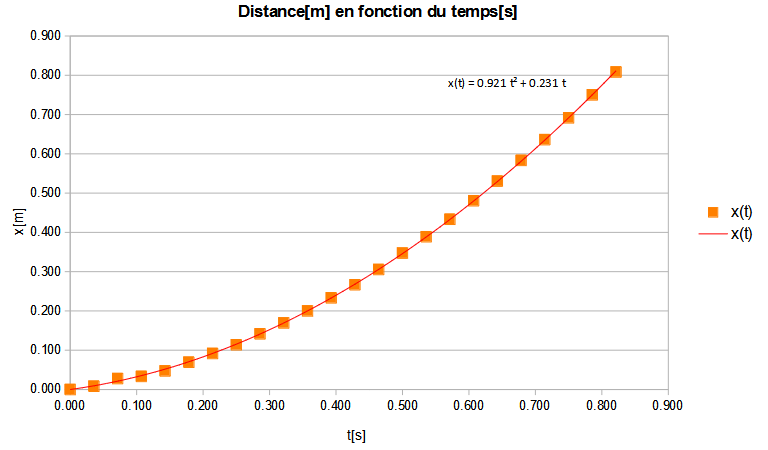
\includegraphics[scale=0.75]{dist tmp.png}
\end{figure}
\begin{figure}[H]
  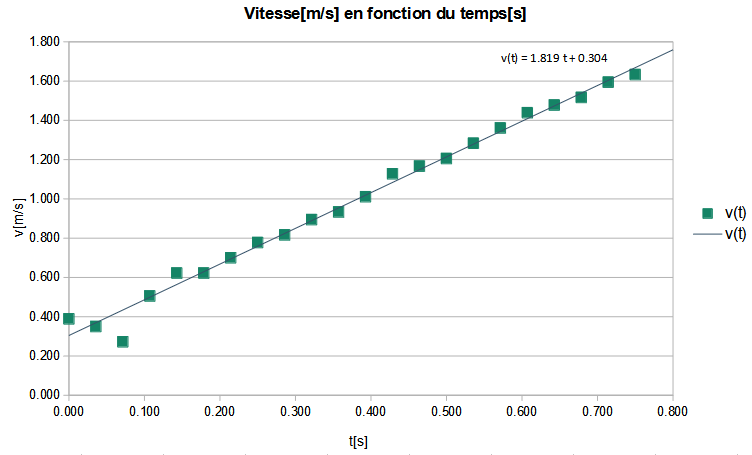
\includegraphics[scale=0.75]{vit tmp.png}
\end{figure}
\end{center}
\clearpage

\section{Analyse des résultats}
\subsection*{Les résultats obtenus correspondent-ils à un MRUA ?}
Malgré quelques mesures pas aussi précises qu’espérées donnant lieu à cause de la propagation de l’incertitude à des vitesses incohérentes avec le reste ($v_m$ au point 1 et 3, possiblement due également au fait que ces points sont peu après le lâché du palet), les courbes de tendances correspondent à un MRUA. En effet, pour la variation de position, cela donne une fonction quadratique et une fonction linéaire pour la variation de vitesse.

\subsection*{Donc, que vaut l’accélération a et la vitesse $v_0$ ?}
Pour connaître $v_0$ et $a$, il suffi de reprendre l’équation horaire de la vitesse $v(t)= v_0+a \cdot t $ et de la comparer avec avec la courbe de tendance $v(t)= 0,304 + 1,819 \cdot t $ et faire de même avec celles de la position, $x(t)=x_0+v_0 \cdot t + \dfrac{1}{2} \cdot a \cdot t^2 $ et $x(t)=0,231 \cdot t + 0,921 \cdot t^2 $. Sachant que $x_0$ vaut 0 (voir tableaux de résultats), voici les valeurs de $a$ et $v_0$ :
\begin{center}
\begin{tabular}{ |>{\columncolor{gray}} l || l |>{\columncolor{lightgray}} l | l | }
\hline
	\rowcolor{gray} \cellcolor{black} & Via $x(t)$ & Via $v(t)$ & Moyenne \\ \hline \hline
	$v_0[m/s]$ & 0.231 & 0.304 & 0.268 \\ \hline
	$a[m/s^2]$ & 1.842 & 1.819 & 1.831 \\ \hline
\end{tabular}
\end{center}
Par voie de conséquence, en injectant tout les résultats obtenus plus haut dans les équations du MRUA, on obtient un modèle assez précis du mouvement du palet :
\begin{center}
$a \approx 1.831 \left[\dfrac{m}{s^2} \right]$\\
$v(t) \approx 0.268 \left[\dfrac{m}{s} \right] + 1.831 \left[\dfrac{m}{s^2} \right] \cdot t $\\
$x(t) \approx 0.268 \left[\dfrac{m}{s} \right] \cdot t + \dfrac{1}{2} \cdot 1.831 \left[\dfrac{m}{s^2} \right] \cdot t^2 $
\end{center}

\section{Conclusion}
Cette expérience a permis l’observation concrète d’un MRUA. Les résultats obtenus sont plutôt cohérents en raison des nombreuses causent d’incertitude (mesures des distances, tailles des taches de lumières et donc repère entre deux points très imprécis, mesure du temps entre deux points, …). Néanmoins, les données ont permis malgré tout de calculer tout les éléments du MRUA impliqués dans l’expérience. Des observations plus précises seraient possibles à l’aide de laser afin de mesurer les distance, soit de cellules et on enregistre le moment de passage dans chaque une d’entre elles, ou quelque chose de moins envisageable, mais qui reste pertinent, comme l’émission d’un court rayon et de mesurer le temps qu’il met à toucher le palais et revenir pendant un intervalle de temps régulier. Cette dernière serait dans le principe pareille à ce qui a été fait mais de manière beaucoup plus précise.

\end{document}